%!TEX root = ../../main.tex
\section{Deep Learning}
\subsection{Einführung}
Viele Probleme oder Aufgaben können heute effizient mit Hilfe eines Computers gelöst werden. Dazu wird in der Regel ein \gls{Algorithmus} verwendet, der die Aufgabe systematisch löst. Es gibt jedoch komplexe Aufgaben, die ein \gls{Algorithmus} nicht lösen kann.

Ein Beispiel hierfür ist die Vorhersage, was ein Kunde in der nächsten Zeit kaufen wird, um ihm entsprechende Vorschläge zu unterbreiten. Probleme dieser Art können nicht mit einem Algorithmus gelöst werden, sondern die Lösung muss aus den vorhandenen Daten ermittelt werden. In solchen Fällen soll der Computer selbst einen Algorithmus erstellen, der dann auf neue Daten angewendet werden kann. Der Computer lernt aus bereits vorhandenen Daten oder Erfahrungen einen Algorithmus zu extrahieren, dabei werden unter anderem Muster und Strukturen erkannt. Mit dem extrahierten Algorithmus kann dann das Kaufverhalten des Kunden approximiert werden. Möglich wird dies durch die enormen Datenmengen, die sich in den letzten Jahren angesammelt haben. Bei jedem Online-Einkauf, beim Aufruf einer Webseite oder beim Öffnen einer App werden Daten erzeugt und gesammelt. Diese Daten können schließlich genutzt werden, um Probleme wie die oben beschriebenen zu lösen.\cite[vgl.][]{Alpaydin2014}

Aufgaben wie das Klassifizieren von Bildern, das Komponieren von Musik\footnote{siehe \cite{GoogleMusicLM} } oder die Generierung von Daten aus Text sind heute mit Deep Learning möglich. Es gibt drei Hauptarten, wie ein Computer lernen kann, die in den Abschnitten \ref{sec:ÜberwachtesLernen}, \ref{sec:UnüberwachtesLernen} und \ref{sec:BestärkendesLernen} beschrieben werden.

\subsection{Überwachtes Lernen}
\label{sec:ÜberwachtesLernen}
Überwachtes Lernen ist ein wichtiger Bereich des maschinellen Lernens, bei dem ein \gls{Modell} anhand von gelabelten Daten lernt. Gelabelt bedeutet, dass den Daten bereits das gewünschte Ergebnis oder der erwartete Wert zugeordnet ist. Ziel des überwachten Lernens ist es, einen \gls{Algorithmus} oder ein \gls{Modell} zu finden, das für neue und noch nicht gesehene Daten die richtigen Labels liefert.\cite[vgl.][]{Frochte2020,IBMSupervisedLearning} \\
Das überwachte Lernen umfasst zwei verschiedene Probleme, die Klassifikation und die Regression. Bei der Klassifikation werden zu Bildern eine oder mehreren Klassen zugeordnet, es können aber auch Texte, Videos oder andere Dinge klassifiziert werden. Ein Beispiel wäre die Klassifizierung von Hunden und Katzen auf Bildern. Dazu wird eine große Anzahl von Bildern von Hunden und Katzen in das \gls{Modell} eingespeist und dieses ordnet den Bildern jeweils die richtigen Klassen zu. Sieht das \gls{Modell} z.B. ein Bild mit einem Hund, so kann es nach dem Training die Klasse ``Hund'' zuordnen. Die meisten E-Mail-Programme verwenden ein solches Klassifikationsmodell, um zwischen seriösen und Spam-E-Mails zu unterscheiden. Das Ergebnis einer Klassifikation ist immer eine Kategorie, die die zu klassifizierenden Daten am besten beschreibt. \\
Der zweite Bereich des maschinellen Lernens ist die Regression, die häufig für Vorhersagen und Prognosen verwendet wird.  Sie ist der Klassifikation ähnlich, aber die Zielmenge ist eine andere. Es wird versucht, Werte für einen meist kontinuierlichen Bereich vorherzusagen, dazu wird der Datensatz mit einer Funktion approximiert. Das Ergebnis einer Regression sind Werte oder Punkte, die die Funktion am besten beschreiben.\cite[vgl.][]{Frochte2020} \\
Im Folgenden geht es hauptsächlich um das überwachte Lernen, genauer gesagt um die Klassifikation. Dabei wird nicht wie im obigen Beispiel ein ganzes Bild klassifiziert, sondern es werden den einzelnen Bildpunkten Klassen zugeordnet.

\subsection{Unüberwachtes Lernen}
\label{sec:UnüberwachtesLernen}
Beim unüberwachten Lernen sind die Daten nicht mit Labels oder Kategorien versehen, wie dies beim überwachten Lernen der Fall ist. Diese Methode des maschinellen Lernens wird eingesetzt, wenn die Beschriftung der Daten nicht ohne weiteres möglich ist. Das \gls{Modell} sucht ohne vorgegebene Kategorien nach Mustern und Strukturen in den Daten. Mit Hilfe statistischer Methoden wird die beste Kategorisierung der Daten gebildet. Das Ergebnis des unüberwachten Lernens sind verschiedene Gruppen von Daten, die jedoch nicht benannt, sondern durchnummeriert werden. Die verschiedenen Daten in den Gruppen haben ähnliche oder gleiche Eigenschaften.\\
Ein gutes Beispiel dafür ist der Bereich ``Kunden kauften auch'' bei Amazon. Hier werden dem Kunden ähnliche Produkte oder Artikel, die oft in Kombination gekauft werden, vorgeschlagen. Es werden keine bestimmten Produktkategorien genannt, sondern nur ähnliche Produkte vorgeschlagen. Es ist schwierig, die Ergebnisse des unüberwachten Lernens zu bewerten, da es keine vergleichbaren Daten mit entsprechenden Annotationen gibt und somit keine Fehler berechnet werden können.\cite[vgl.][]{Lang2023,Frochte2020}


\subsection{Bestärkendes Lernen}
\label{sec:BestärkendesLernen}
Oft gibt es Probleme, bei denen nicht genau festgestellt werden kann, ob etwas richtig oder falsch ist. Die Daten für solche Probleme, sofern vorhanden, sind daher nicht beschriftet. Es ist jedoch möglich zu sagen, ob die Ergebnisse zur Lösung des Problems geeignet sind oder nicht, in diesen Fällen kommt bestärkendes Lernen zum Einsatz. In der Robotik ist bestärkendes Lernen ein klassischer Anwendungsfall. Für Roboter stehen in der Regel keine Trainingsdaten zur Verfügung, so dass der Roboter selbst lernen muss, was gut und was schlecht ist. \cite[vgl.][]{Ertel2021} \\
Ziel des Roboters ist es, eine geeignete Lösung oder Strategie für das Problem zu finden. Beim bestärkenden Lernen spricht man oft von sogenannten Agenten, die darauf trainiert werden, ein Problem zu lösen. Auf der Suche nach einer geeigneten Strategie werden diese kontinuierlich für gute und schlechte Aktionen belohnt oder bestraft. Ein einfaches Beispiel wäre ein Saugroboter, der in einem Hotel die Zimmer saugt. In den Zimmern, in denen der Roboter z.B. nichts umgestoßen hat, wird er belohnt. Stößt der Roboter etwas um oder saugt etwas Unerwünschtes auf, wird er bestraft. \cite[vgl.][]{Frochte2020} Das Belohnungssystem kann auf Punkten basieren, so dass der Saugroboter im positiven Fall Pluspunkte und im negativen Fall Minuspunkte erhält und sein Verhalten entsprechend anpasst.

\subsection{Künstliches Neuronales Netz}
Die Struktur und Funktion des menschlichen Gehirns ist das Vorbild für künstliche neuronale Netze. Sie bestehen aus einer Vielzahl von künstlichen Neuronen, die miteinander verbunden sind und Informationen verarbeiten. Ein \ac{KNN} wird für verschiedene Anwendungen wie Mustererkennung, Datenanalyse oder Vorhersagen eingesetzt.

\subsubsection{Biologisches Neuron}

\begin{figure}[h]
	\centering
	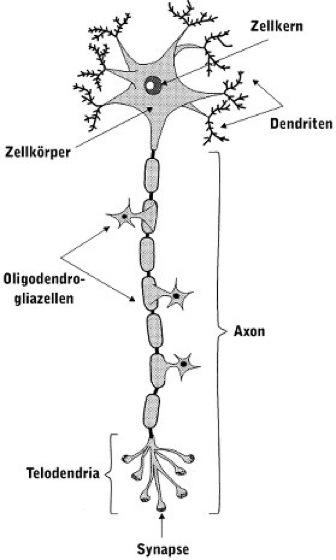
\includegraphics[width=.4\textwidth]{biologisches_neuron.jpg}
	\caption{Aufbau biologisches eines biologischen Neurons (Quelle: \url{https://www.spektrum.de/lexikon/psychologie/neuron/10516})}		\label{fig:BioNeuron}
\end{figure}

Das biologische Neuron (siehe Abb. \ref{fig:BioNeuron}) ist das Vorbild für künstliche Neuronen. Es besteht aus Dendriten, die elektrische Signale von anderen Nervenzellen aufnehmen und an den Zellkörper weiterleiten. 
Im Axonhügel, der sich zwischen Zellkörper und Axon befindet, werden die elektrischen Signale gesammelt und summiert. Erst wenn ein bestimmter Schwellenwert überschritten ist, wird das Signal an das Axon weitergeleitet. Der Schwellenwert verhindert, dass sehr kleine Signale, die keine Relevanz haben, weitergeleitet werden. Ohne diese Signalfilterung wäre eine Verarbeitung der relevanten Signale nicht möglich. Das Signal, das schließlich über das Axon zu den Synapsen transportiert wird, heißt Aktionspotenzial. An die Synapsen schließen sich weitere Dendriten der Nervenzellen an und empfangen die weitergeleiteten Signale. Ein biologisches Neuron kann dabei bis zu mehrere tausend Verbindungen zu anderen Neuronen haben, die wiederum entsprechend viele Verbindungen haben können.\cite[vgl.][]{Posthoff2022,JuergenCleve2020}

\subsubsection{Künstliches Neuron}
\label{subsubsec:KünstlichesNeuron}
\begin{figure}[ht]
	\centering
	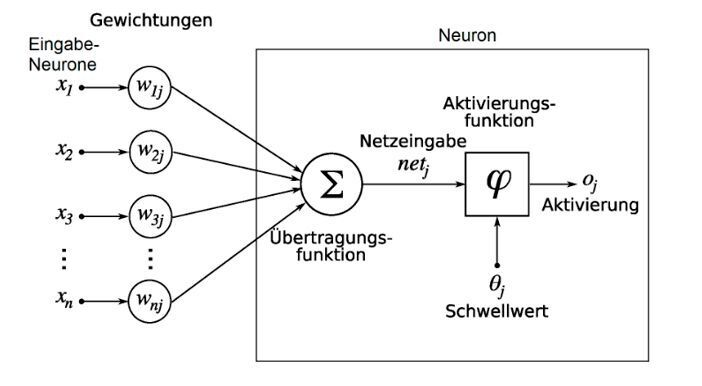
\includegraphics[width=.8\textwidth]{kunstliches_neuron.jpg}
	\caption{Schema eines künstlichen $Neurons_j$ (Quelle: \url{https://www.dev-insider.de/grundbegriffe-und-einfache-beispiele-a-864507/})}
	\label{fig:KünstlichesNeuron}
\end{figure}
Ein künstliches Neuron ist ein mathematisches Modell, das die Funktion eines biologischen Neurons nachahmt. Das künstliche Neuron in Abb. \ref{fig:KünstlichesNeuron} besitzt Eingänge $x_n$, die mit den Dendriten des biologischen Neurons vergleichbar sind. Die Eingangsinformationen können von anderen Neuronen oder aus der Umgebung stammen. \\
Bevor die Eingangsinformationen in das Neuron gelangen, werden sie mit einem Gewicht $w_{nj}$ multipliziert. Anschließend werden die Eingaben mit Hilfe einer Übertragungsfunktion (Propagationsfunktion) verknüpft, d.h. die Werte werden aufsummiert. Das summierte Ergebnis ist die Netzeingabe $net_j$, der die Informationen zusammenfasst, die in das Neuron eingehen. Die Aktivierungsfunktion berechnet die Aktivierung $o_j$, die abhängig vom Schwellenwert $\theta_j$ an alle angeschlossenen Neuronen weitergegeben wird. \cite[vgl.][]{JuergenCleve2020}

\subsubsection{Das Perzeptron}
Das Perzeptron ist ein einfaches künstliches neuronales Netz, das von Frank Rosenblatt als Modell vorgestellt wurde. Als Beispiel wird ein Photo-Perzeptron beschrieben, das in der Lage ist, einfache visuelle Muster zu erkennen. Es besteht aus der Retina (Netzhaut), der Assoziationsschicht und der Ausgabeschicht. Die Retina liefert binäre Eingangswerte, die über gewichtete Verbindungen an die Assoziationsschicht weitergeleitet werden. Die Neuronen der Retina sind fest mit den Neuronen der Abbildungsschicht verbunden, aber nicht alle Neuronen sind miteinander verbunden. Die Verbindungen zwischen der Abbildungsschicht und der Ausgabeschicht sind dagegen variabel. Während des Trainings, also des Lernens, werden die Gewichtungen zwischen ihnen angepasst. \\
Beim Training werden dem Perzeptron verschiedene Beispiele gezeigt, anhand derer es lernen soll. Ein Beispiel besteht immer aus einem Eingangsvektor $x$ und einem Ausgangsvektor $y$. Die Aufgabe des Perzeptrons ist es, durch Anpassung der internen Werte zu jedem Eingabevektor $x$ einen passenden Ausgabevektor $y$ zu erzeugen. Ziel des Trainings ist es, bisher nicht gesehenen, aber ähnlichen Eingabevektoren $x'$ ebenfalls einen passenden Ausgabevektor $y$ zuzuordnen, man spricht in diesem Fall von Generalisierung. \cite[vgl.][]{Scherer1997} \\
Die Struktur des Perzeptrons schränkt jedoch die Klassifikation von Daten ein. Es ist nur in der Lage, linear separierbare Datenmengen zu trennen. Das heißt, die Datenmenge kann durch eine gegebene Gerade in zwei separate Datenmengen getrennt werden. Die Ausgänge des Perzeptrons sind also auf 0 oder 1 beschränkt, wobei nicht alle Datenmengen trennbar sind, sondern nur solche, deren Trenngerade durch den Ursprung geht.\cite{Ertel2021}

\subsubsection{Aufbau}
Der klassische Aufbau eines Neuronalen Netzes besteht aus einer Eingabeschicht (engl.: Input Layer), einer oder mehreren verborgenen Schichten (engl.: Hidden Layer) und der Ausgabeschicht (engl.: Output Layer). Die Eingabeschicht nimmt Werte aus der Umgebung auf und leitet sie an die versteckte Schicht weiter, von wo aus sie an weitere versteckte Schichten oder an die Ausgabeschicht, die das Endergebnis ausgibt, weitergeleitet werden. Die Verbindungen der Neuronen zwischen den verschiedenen Schichten haben Gewichtungen, mit denen die eingehenden Werte multipliziert werden. Die Komplexität der Struktur hängt von der Anzahl der Neuronen und Schichten ab. \cite[vgl.][]{Frochte2020}


\subsubsection{Training eines Neuronalen Netzes}
Das Training eines neuronalen Netzes ist ein wesentlicher Aspekt des Deep Learning, bei dem die Anpassungen der Gewichte und Schwellenwerte innerhalb des Netzes erfolgen. Das Training kann je nach Art und Menge der Daten mehrere Stunden oder sogar Tage dauern. Ein neuronales Netz gilt als trainiert, wenn es zu einem Eingabevektor $x$ zuverlässig einen passenden Ausgabevektor $y$ bestimmen kann. Das Netz ist dann in der Lage, auch bisher unbekannten Eingabevektoren $x'$ passende Ausgabevektoren $y'$ zuzuordnen. \cite[vgl.][]{Scherer1997}

Ein entscheidendes Konzept beim Training ist die Fehler- oder Verlustfunktion (engl.: Loss), die im Abschnitt  \ref{subsec:AktivierungsfunktionenVerlust-FunktionenOptimierer} genauer beschrieben wird und die Differenz zwischen den vorhergesagten und den tatsächlichen Ergebnissen vergleicht und einen Fehler berechnet. Ziel des Trainings ist es, die Verlustfunktion durch Anpassung der internen Parameter des neuronalen Netzes zu minimieren. Die Parameter des Netzes werden zu Beginn des Trainings zufällig initialisiert und während des Trainings schrittweise angepasst. \cite[vgl.][]{Choo2020}\\
Die Rückwärtspropagation (engl.: Backpropagation) ist ein weit verbreitetes Lernverfahren für Neuronale Netze, das auf der oben genannten Fehlerminimierung basiert. Bei der Backpropagation wird im Allgemeinen die Delta-Lernregel verwendet, die besagt, dass die Fehlerminimierung durch Änderung eines Gewichts $w_{ij}$ einen Gradientenabstieg anstrebt. Der Ausgangspunkt dieser Lernregel ist wie folgt definiert
\begin{equation}
	\Delta_{p}w_{ij} \equiv -\dfrac{dE_p}{dw_{ij}}
\end{equation}
$\Delta_{p}w_{ij}$ entspricht dabei der Änderung eines Gewichts zwischen $i$ und $j$. $dE_p$ ist der gemessene Fehler innerhalb der Lernmenge und $dw_{ij}$ ist die Gewichtung der Neuronen von der Schicht $i$ zur Schicht $j$. \cite[vgl.][]{Rumelhart1986}

Der Backpropagation-Algorithmus besteht im Wesentlichen aus zwei Schritten, der Vorwärtspropagation und der Rückwärtspropagation.
Der erste Schritt ist die Vorwärtspropagation, bei der die Eingabevektoren durch das Netzwerk verarbeitet werden. Die Eingaben werden von Schicht zu Schicht weitergeleitet und durch die Gewichtungen und Aktivierungsfunktionen transformiert. Am Ende dieses Schrittes steht eine Ausgabe, die für den zweiten Schritt verwendet wird. \\
Im nächsten und letzten Schritt des Trainings, der Rückwärtspropagation, wird die Ausgabe mit dem tatsächlich erwarteten Wert verglichen und anschließend aus der Differenz zwischen Soll- und Istwert ein Fehler berechnet. Als Beispielfunktion für die Berechnung eines Fehlers kann der in Gleichung \ref{eq:mse} definierte mittlere quadratische Fehler (MSE) verwendet werden.
\begin{equation}
	\label{eq:mse}
	E = \dfrac{1}{2} \sum (Y_i - \hat{Y}_{i})^2
\end{equation}
Nach der Fehlerberechnung werden die Fehler für die Neuronen der einzelnen Schichten bestimmt. Dabei wird der Beitrag jedes Neurons zum Gesamtfehler berechnet. Anschließend wird die Gewichtung eines Neurons anhand seines Fehlers angepasst. Die Gewichte werden mit einem konstanten Faktor $\nu$ und einem weiteren Term in Abhängigkeit vom Fehler multipliziert. Dieser Prozess wird iterativ wiederholt, bis der Fehler auf ein geeignetes Minimum reduziert wurde. Ist der Fehler auf ein Minimum gesunken und ändert sich nicht mehr wesentlich, so spricht man von einer Konvergenz des \gls{Modell} und das Training kann beendet werden.\cite[vgl.][]{Scherer1997}

\subsection{Aktivierungsfunktionen, Verlust-Funktionen und Optimierer}
\label{subsec:AktivierungsfunktionenVerlust-FunktionenOptimierer}
Für das Training und die generelle Funktionalität eines Neuronalen Netzes werden noch einige Komponenten benötigt.\
Eine Komponente ist die bereits im Abschnitt \ref{subsubsec:KünstlichesNeuron} erwähnte Aktivierungsfunktion. Sie berechnet die Aktivierung $o_j$, die abhängig von einem Schwellwert $\theta_j$ an die nachgeschalteten Neuronen weitergegeben wird. Wird der Schwellenwert $\theta_j$ nicht überschritten, wartet das Neuron auf weitere Eingangssignale und wiederholt die Berechnung der Aktivierung $o_j$, bis der Schwellenwert $\theta_j$ überschritten wird und das Neuron seine Ausgabe weitergibt. Es gibt verschiedene Aktivierungsfunktionen für unterschiedliche Zwecke.

Die Identitätsfunktion ist eine einfache Aktivierungsfunktion, die eine lineare Abbildung der Eingabe auf die Ausgabe liefert. Sie eignet sich für einfache Aufgaben, wird die Problemstellung komplexer, sind nichtlineare Aktivierungsfunktionen wie Tangens hyperbolicus, \ac{ReLU} oder Sigmoid besser geeignet. Je nach Anwendung und Bedarf wird eine geeignete Funktion ausgewählt. Die Sigmoidfunktion normalisiert die Ausgaben eines Netzes auf den Bereich zwischen 0 und 1, während der Tangens hyperbolicus die Werte in den Bereich zwischen -1 und 1 bringt. Die Funktion \ac{ReLU} verhält sich etwas anders als die vorhergehenden Funktionen, da sie für alle positiven Werte die entsprechenden Ausgaben und für alle negativen Werte den Wert 0 zurückgibt. Eine weitere erwähnenswerte Aktivierungsfunktion ist die Softmax-Funktion, die ebenfalls Werte in einen Bereich zwischen 0 und 1 transformiert, jedoch eine Wahrscheinlichkeitsverteilung darstellt. Die Besonderheit der Softmax-Funktion liegt darin, dass sich alle Ausgaben zu 1 addieren und somit die Ausgabewerte als Wahrscheinlichkeiten interpretiert werden können. \cite[vgl.][]{Frick2021}\\
Eine weitere Komponente ist die Verlustfunktion, die für das Training eines Neuronalen Netzes essentiell ist. Diese hat zum Ziel, den Fehler, auch Verlust genannt, den ein Netz bei einer Vorhersage produziert, zu minimieren. Ein Fehler tritt auf, wenn das Netz eine falsche oder andere Ausgabe als die erwartete erzeugt. Um den Gesamtfehler eines Netzes zu berechnen, werden die Ausgaben des neuronalen Netzes mit den erwarteten Ergebnissen verglichen. Die Verlustfunktion hilft, die Differenz zu quantifizieren und den Gesamtfehler des Netzes zu berechnen. \cite{Frick2021}\\
Wie bei den Aktivierungsfunktionen gibt es je nach Art der Aufgabe verschiedene Verlustfunktionen, wie z.B. Binary Cross Entropy (BCE), Categorical Cross Entropy oder Mean Squared Error. Die Binary Cross Entropy wird für binäre Klassifikationsprobleme verwendet, wie z.B. die Unterscheidung von seriösen und Spam-E-Mails, während die Categorical Cross Entropy für Probleme mit mehr als zwei Klassen verwendet wird. Die Wahl der Verlustfunktion hängt also auch von der Ausgabe des Netzes ab. 

Die letzte wesentliche Komponente ist der Optimierer, der die Gewichte und Biases anpasst, um Fehler zu minimieren und die Leistung des Netzes zu verbessern. Biases sind zusätzliche Konstanten, mit denen ein Neuron versorgt wird und die bei der Berechnung der Ausgabe eine Rolle spielen. Der Bias erhöht die Fähigkeit des Netzes, komplexe Beziehungen zwischen Eingaben und Ausgaben zu modellieren, und kann so auch nichtlineare Beziehungen erkennen. \\
Es gibt verschiedene Arten von Optimierungsalgorithmen, der am weitesten verbreitete Algorithmus ist der \ac{SGD}, der auch die Grundlage für weitere Optimierungsverfahren bildet. Der \ac{SGD} aktualisiert Gewichte und Bias auf der Basis der Ableitung der Verluste. Zur Beschleunigung der Berechnung wird eine Zufallsstichprobe aus dem Trainingsdatensatz verwendet. \cite[vgl.][]{Goodfellow2016} \\
Ein weiterer Optimierungsalgorithmus ist Adam, der eine Erweiterung von \ac{SGD} ist und eine adaptive Lernrate verwendet, um die internen Parameter des Netzes anzupassen. Durch die adaptiven Lernraten erreicht der Algorithmus eine schnellere Konvergenz und eine höhere Genauigkeit als der \ac{SGD}. \cite[vgl.][]{Kingma2014}

\subsection{\acf{CNN}}
\acf{CNN} sind eine spezielle Form von Neuronalen Netzen, die Bilddaten verarbeiten können. Sie erkennen mit Hilfe verschiedener Filter Muster, Strukturen und Geometrien in Bildern und können diese klassifizieren. Im folgenden Abschnitt wird der Aufbau und die Funktionsweise eines \ac{CNN}s erläutert, wobei auf die verschiedenen Schichten innerhalb des Netzes sowie auf die mathematische Operation Faltung (engl.: Convolution) eingegangen wird.

\begin{figure}[ht]
	\centering
	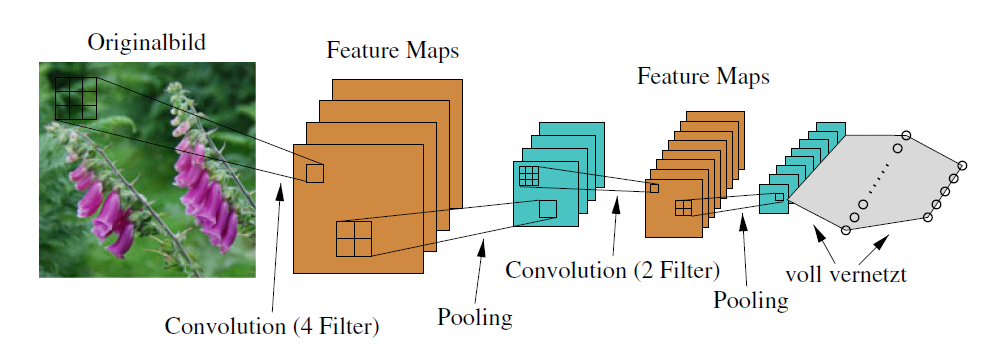
\includegraphics[width=.9\textwidth]{cnn_aufbau.png}
	\caption{Ein \ac{CNN} mit zwei Faltungs-Schichten gefolgt von je einer Pooling-Schicht und am Ende
		zwei voll vernetzten Schichten (Quelle: \cite{Ertel2021})}	
	\label{fig:cnn_aufbau}
\end{figure}

Der Aufbau eines \ac{CNN} besteht aus mehreren Faltungs-, Pooling- und vollvernetzten Schichten, wie in Abbildung \ref{fig:cnn_aufbau} dargestellt

\paragraph{Convolutional-Layer} ist die Faltungsschicht, die in der Lage ist, Merkmale wie Linien, Kanten und geometrische Formen in Bildern zu erkennen und zu extrahieren. Bei einer Faltung wandert ein Filter (engl.: Kernel) über das Eingabebild und erzeugt so ein neues Bild, auch Feature-Maps genannt. Mathematisch gesehen wandert der Filter über eine Funktion statt über ein Bild und erzeugt so ein neues Bild. Bei der Faltung eines Bildes wird meist ein Filter in Form einer 2D-Matrix verwendet, wie in Gleichung \ref{eq:kernel} als Beispiel dargestellt. Die Werte des Filters werden zu Beginn zufällig bestimmt und während des Trainings angepasst.
\begin{equation}
\begin{bmatrix}
	1 & 2 & 3 \\
	4 & 5 & 6 \\
    7 & 8 & 9
\end{bmatrix}
\label{eq:kernel}
\end{equation}
Der Filter wird schrittweise über das Eingabebild bewegt, wobei jedes Filterelement mit dem darunterliegenden Pixel des Eingabebildes multipliziert und dann aufsummiert wird. Die Summe ist dann das Ergebnis des neuen Bildpunktes. Die Schrittweite des Filters wird ``Stride'' genannt und gibt an, um wie viele Bildpunkte (Pixel) der Filter verschoben wird. Bei einer 2D-Faltung können zwei Werte für den Stride angegeben werden, die Verschiebung in Richtung der X-Achse und die Verschiebung in Richtung der Y-Achse. Die Gleichung \ref{eq:conv_result} gibt das Ergebnis einer Faltung mit dem Ausdruck aus \ref{eq:conv} an.

\begin{equation}
	\begin{pmatrix}
		a_{11} & a_{12} & a_{13} \\
		a_{21} & a_{22} & a_{23} \\
		a_{31} & a_{32} & a_{33}
	\end{pmatrix}
	*
	\begin{pmatrix}
		w_{11} & w_{12} \\
		w_{21} & w_{22}
	\end{pmatrix}
	\label{eq:conv}
\end{equation}

\begin{equation}
	\begin{pmatrix}
		(a_{11}w_{11} + a_{12}w_{12} + a_{21}w_{21} + a_{22}w_{22}) & (a_{12}w_{11} + a_{13}w_{12} + a_{22}w_{21} + a_{23}w_{22}) \\
		(a_{21}w_{11} + a_{22}w_{12} + a_{31}w_{21} + a_{32}w_{22}) & (a_{22}w_{11} + a_{23}w_{12} + a_{32}w_{21} + a_{33}w_{22}) \\
	\end{pmatrix}
	\label{eq:conv_result}
\end{equation}

Es ist zu beachten, dass das Ergebnis in \ref{eq:conv_result} kleiner ist als das Originalbild. Dies liegt daran, dass kein Padding verwendet wurde, um die Ränder des Eingabebildes aufzufüllen. Die Größe der Ergebnismatrix kann mit der Gleichung \ref{eq:conv_size} berechnet werden, wobei $W$ die Eingabegröße des Bildes, $F$ die Filtergröße, $S$ der Stride und $P$ das Padding ist. \cite[vgl.][]{Teoh2023}

\begin{equation}
	W_{out}= \dfrac{W+2P-F}{S}+1
	\label{eq:conv_size}
\end{equation}

\paragraph{Pooling-Layer} dient der Extraktion von Bildmerkmalen (engl.: features), die eine hohe semantische Bedeutung haben. Die Eingangsdaten dieser Schicht sind die Ausgangsdaten der vorhergehenden Faltungsschicht. Diese Schicht verwendet entweder das Maximum- oder das Average-Pooling. Dabei werden überflüssige und redundante Informationen aus dem Datensatz entfernt. Durch das Entfernen der unwesentlichen Bestandteile wird die Rechenzeit reduziert und die Merkmale werden verdichtet. 

Beim Pooling wird ebenfalls ein Filter, in der Regel der Größe $2\times2$, mit einer Schrittweite von zwei über das Bild bewegt. In Abbildung \ref{fig:pooling} werden beide Arten des Poolings durchgeführt. Das Max-Pooling extrahiert jeweils den höchsten Wert, der innerhalb der Filtermatrix liegt. Das Average-Pooling nimmt jeweils den Mittelwert aller Elemente innerhalb der Filter-Matrix. Durch das Pooling verkleinert sich das Bild je nach Filtergröße und Schrittweite.\cite[vgl.][]{Teoh2023} Im Beispiel der Abbildung \ref{fig:pooling} wird das Ausgangsbild um die Hälfte verkleinert, die Größe nach dem Pooling berechnet sich ebenfalls nach der Formel aus \ref{eq:conv_size}.

\paragraph{Fully-Connected-Layer} oder vollständig verknüpfte Schicht, bildet den Abschluss eines \ac{CNN}s. Die Merkmale der vorhergehenden Schicht, also der Pooling-Schicht, werden hier mit allen Ausgabemerkmalen verknüpft, es handelt sich also um ein normales Neuronales Netz. 

Zunächst muss aus der Ausgabe der vorhergehenden Schicht eine 1D-Matrix erzeugt werden, dieser Vorgang wird auch ``flatten'' genannt. Anschließend wird jedes Element der 1D-Matrix mit jedem Element der Ausgabeschicht verbunden. Die Ausgabe des Netzes zeigt dann z.B. die Klassifikation eines Bildes, indem berechnet wird, welches Ausgabeelement die höchste Wahrscheinlichkeit hat. \cite[vgl.][]{Weidman2020}

\begin{figure}
	\centering
	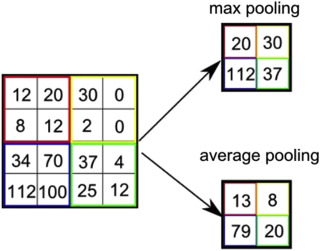
\includegraphics[width=.6\textwidth]{pooling.jpg}
	\caption{Maximal und Mittelwert-Pooling, sowie das Ergebnis der beiden Methoden. (Quelle: \url{https://www.sciencedirect.com/topics/mathematics/pooling-layer})}
	\label{fig:pooling}
\end{figure}


\subsection{Over- und Underfitting}
Over- und Underfitting sind zwei Probleme, die beim Training eines neuronalen Netzes auftreten können. Diese Probleme beeinflussen die Generalisierungsfähigkeit des Modells, d.h. die Fähigkeit, auf neuen, bisher nicht gesehenen Daten gute Ergebnisse zu erzielen.
Overfitting tritt auf, wenn ein Modell zu stark an die Trainingsdaten angepasst ist und dadurch keine allgemeinen Strukturen mehr erkennt. In diesem Fall hat sich das \gls{Modell} die Trainingsdaten eingeprägt und ist daher nicht in der Lage, auf neuen Daten gute Ergebnisse zu erzielen. Ist die Kapazität des \gls{Modell}s zu groß, neigt das Neuronale Netz dazu, kleine Variationen in den Daten zu lernen und verliert dadurch die Generalisierung der Daten.\\
Beim Underfitting hingegen ist das \gls{Modell} nicht in der Lage, eine zugrundeliegende Struktur in den Daten zu erkennen, was zu einer schlechten Leistung sowohl bei den Trainings- als auch bei den Testdaten führt. Beim Underfitting hat das \gls{Modell} meist eine zu geringe Kapazität, um alle relevanten Informationen zu speichern.\cite[vgl.][]{Goodfellow2016}